Dette afsnit kommer til at handle om hvilken slags valuta, som kan tages i brug af lommepengemodellerne. Der bliver argumenteret for eventuelle fordele og ulemper, ved de valuta former som er tilgængelige.

Systemet kan fungere mere i en retning der ligner et spil, hvor de penge, der er i omløb, ikke har nogen relevans til virkelige penge. Altså, der bliver gjort brug af en form for valuta inden for systemet, og børnene kan derefter handle med denne form for valuta, som de nu engang ønsker. På den anden side kan systemet også gøre brug af rigtige penge, i form af lommepenge, idet systemet allerede er forbundet med pligter og evt. andet i husholdningen.

\begin{figure}[htb]
\centering
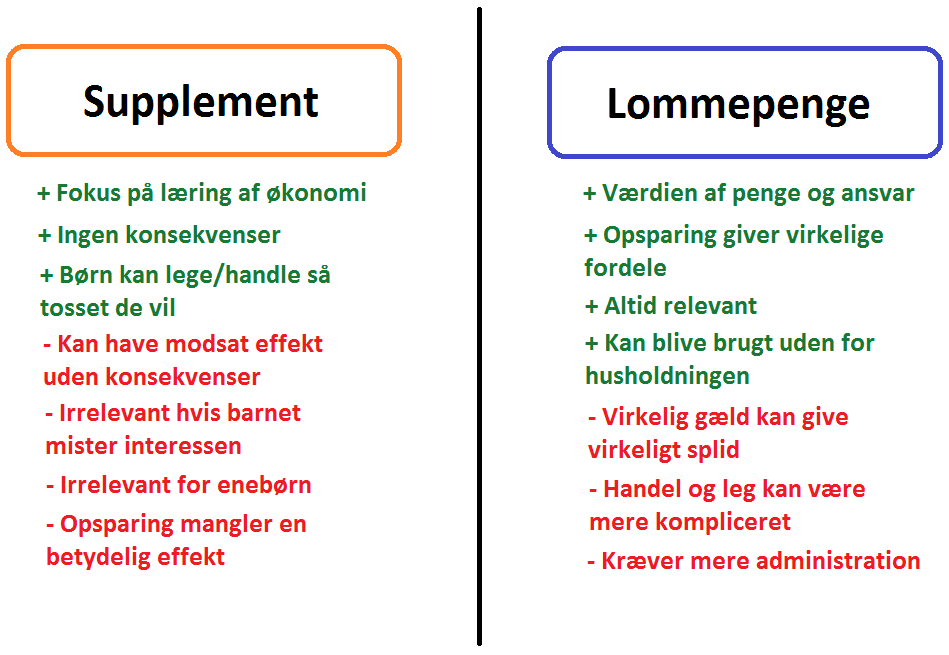
\includegraphics[width=0.8\textwidth]{Billeder/supplomme.png}
\caption{Fordele og Ulemper ved de to valuta former}
\label{SuppLomme}
\end{figure}

Systemet, som er baseret på sin egen valuta, kan have nogle fordele, når det kommer til at lære børn og unge omkring økonomi. Idet at systemet gør brug af sin egen fiktive valuta, som ikke har nogen sammenhæng med virkelige penge, så er der ingen større konsekvenser ved lån og minus på kontoen, som ellers ville være tilfældet med virkelige penge. Børnene kan derfor lege med systemet, og handle med hinanden, som de nu engang lyster. På den måde kan de også lære forskellige aspekter ved økonomi.

Det kan dog være, idet at der ikke er nogen konsekvenser ved systemet, at det kan have den modsatte effekt på barnet.  Systemet kan ende med at blive set mere som et middel i børnenes leg, i stedet for et værktøj til at lære dem om økonomi. På samme måde kan systemet ende med at blive irrelevant, hvis børnene mister interessen. Denne form for system, som fungerer som et supplement til lommepengene, vil have stor fokus på handlen der bliver gjort mellem børnene i dette system. Derfor vil systemet være stort set irrelevant for enebørn, som ikke har nogen søskende at handle med. Dette vil dog ikke være tilfældet hvis det er muligt at inkludere forældrene i systemet, og derfor også handlen. På samme måde mangler opsparing også en betydelig effekt, da det er en fiktiv valuta, og ville ellers bremse handlen og legen.
 
På den anden side har man et system, som er baseret omkring rigtige penge og er forbundet med de lommepenge, som børnene ellers ville have fået. Sådan et system, som sætter pengene sammen med opfyldelse af pligter, og giver rigtige penge der kan bruges uden for husholdningen, kan give en større fornemmelse af ansvar og den virkelige værdi af penge. Systemet kan ende med at give konstruktive lektioner angående økonomi, idet aspekter som renter og opsparing vil have en meget virkelig effekt. Denne form for system vil næsten altid være relevant, og vil sikkert kun blive mere relevant som barnet bliver ældre.

Ulemperne ved dette system kan være, at det muligvis vil give splid i husholdningen, idet at gælden i systemet er baseret på virkelige penge. Handlen mellem søskende bliver også mere kompliceret, fordi der er virkelige penge på bordet, og det giver heller ikke børnene den samme frihed for leg, som supplementsystemet har. Systemet baseret på penge kræver i sidste ende mere administration fra forældrenes side, sådan at børnene ikke ender med at sætte sig i gæld til skuldrene som 7-årige, udnytter sine muligvis yngre søskende, eller misbruger systemet.
 
